\documentclass[aspectratio=169,12pt]{beamer}
\usetheme{Madrid}
\usecolortheme{whale}
\usepackage{graphicx}
\usepackage{tikz}
\usepackage{listings}
\usepackage{booktabs}
\usepackage{xcolor}

% Define colors
\definecolor{clinblue}{RGB}{52,152,219}
\definecolor{clinred}{RGB}{231,76,60}
\definecolor{clingreen}{RGB}{46,204,113}
\definecolor{clinorange}{RGB}{243,156,18}
\definecolor{clinpurple}{RGB}{155,89,182}

% Set theme colors
\setbeamercolor{structure}{fg=clinblue}
\setbeamercolor{frametitle}{bg=clinblue,fg=white}
\setbeamercolor{title}{bg=clinblue,fg=white}

% Code listing style
\lstset{
    basicstyle=\ttfamily\small,
    keywordstyle=\color{clinblue}\bfseries,
    commentstyle=\color{gray},
    stringstyle=\color{clingreen},
    numbers=none,
    breaklines=true,
    frame=single,
    rulecolor=\color{gray!30}
}

\title{\textbf{ClinOrchestra v1.0.0}}
\subtitle{Universal, Autonomous Clinical AI Platform\\for Task-Driven LLM Orchestration}
\author{Frederick Gyasi}
\institute{Medical University of South Carolina\\Biomedical Informatics Center}
\date{\today}

\begin{document}

% Title Frame
\begin{frame}
\titlepage
\end{frame}

% Outline
\begin{frame}{Outline}
\tableofcontents
\end{frame}

% ========================================
% SECTION 1: OVERVIEW & MOTIVATION
% ========================================
\section{Overview \& Motivation}

\begin{frame}{The Challenge}
\begin{columns}[T]
\column{0.5\textwidth}
\textbf{Clinical Data Extraction Problems:}
\begin{itemize}
    \item Unstructured clinical narratives
    \item Variable documentation styles
    \item Domain-specific knowledge required
    \item Manual curation is slow \& expensive
    \item Hardcoded systems lack flexibility
\end{itemize}

\column{0.5\textwidth}
\textbf{Existing Solutions Fail Because:}
\begin{itemize}
    \item \textcolor{clinred}{Task-specific implementations}
    \item \textcolor{clinred}{Manual tool selection}
    \item \textcolor{clinred}{Limited scalability}
    \item \textcolor{clinred}{No autonomous reasoning}
    \item \textcolor{clinred}{Poor performance}
\end{itemize}
\end{columns}

\vspace{0.3cm}
\begin{alertblock}{Critical Need}
\textbf{Universal, autonomous platform} that adapts to ANY clinical task through LLM orchestration
\end{alertblock}
\end{frame}

\begin{frame}{The ClinOrchestra Solution}
\begin{block}{Core Innovation}
\textbf{Task-driven autonomous orchestration} - not hardcoded logic
\end{block}

\begin{columns}[T]
\column{0.33\textwidth}
\centering
\textcolor{clinblue}{\Large\textbf{Universal}}\\[0.2cm]
\small
Adapts to ANY clinical task\\
No task-specific code\\
User-defined prompts\\
Custom tools \& schemas

\column{0.33\textwidth}
\centering
\textcolor{clingreen}{\Large\textbf{Autonomous}}\\[0.2cm]
\small
LLM decides tools\\
Self-correcting execution\\
Adaptive strategies\\
Intelligent orchestration

\column{0.33\textwidth}
\centering
\textcolor{clinorange}{\Large\textbf{Production-Ready}}\\[0.2cm]
\small
400x cache speedup\\
60-75\% async gains\\
Multi-GPU support\\
Robust error handling
\end{columns}

\vspace{0.5cm}
\begin{center}
\fbox{\parbox{0.9\textwidth}{\centering
\textbf{Examples} (malnutrition, ADRD) demonstrate \textit{capability}, not \textit{limits}
}}
\end{center}
\end{frame}

% ========================================
% SECTION 2: ARCHITECTURE
% ========================================
\section{System Architecture}

\begin{frame}{6-Layer Modular Architecture}
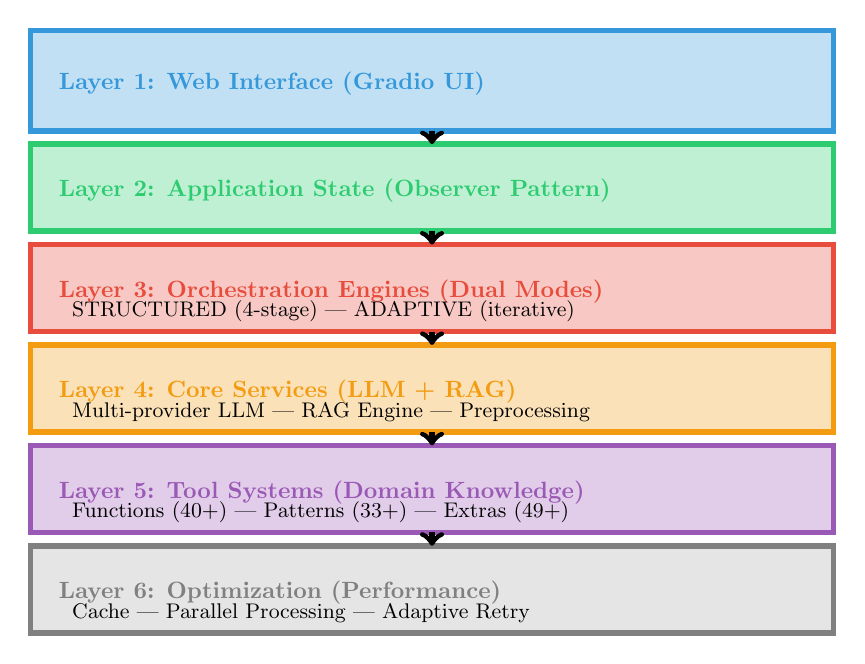
\begin{tikzpicture}[scale=0.85, every node/.style={transform shape}]
    % Layer 6 - UI
    \draw[fill=clinblue!30, draw=clinblue, line width=2pt] (0,9) rectangle (12,10.5);
    \node[anchor=west, font=\bfseries] at (0.3,9.7) {\textcolor{clinblue}{Layer 1: Web Interface (Gradio UI)}};

    % Layer 5 - State
    \draw[fill=clingreen!30, draw=clingreen, line width=2pt] (0,7.5) rectangle (12,8.8);
    \node[anchor=west, font=\bfseries] at (0.3,8.1) {\textcolor{clingreen}{Layer 2: Application State (Observer Pattern)}};

    % Layer 4 - Agents
    \draw[fill=clinred!30, draw=clinred, line width=2pt] (0,6) rectangle (12,7.3);
    \node[anchor=west, font=\bfseries] at (0.3,6.6) {\textcolor{clinred}{Layer 3: Orchestration Engines (Dual Modes)}};
    \node[anchor=west, font=\small] at (0.5,6.3) {STRUCTURED (4-stage) | ADAPTIVE (iterative)};

    % Layer 3 - Core Services
    \draw[fill=clinorange!30, draw=clinorange, line width=2pt] (0,4.5) rectangle (12,5.8);
    \node[anchor=west, font=\bfseries] at (0.3,5.1) {\textcolor{clinorange}{Layer 4: Core Services (LLM + RAG)}};
    \node[anchor=west, font=\small] at (0.5,4.8) {Multi-provider LLM | RAG Engine | Preprocessing};

    % Layer 2 - Tools
    \draw[fill=clinpurple!30, draw=clinpurple, line width=2pt] (0,3) rectangle (12,4.3);
    \node[anchor=west, font=\bfseries] at (0.3,3.6) {\textcolor{clinpurple}{Layer 5: Tool Systems (Domain Knowledge)}};
    \node[anchor=west, font=\small] at (0.5,3.3) {Functions (40+) | Patterns (33+) | Extras (49+)};

    % Layer 1 - Optimization
    \draw[fill=gray!20, draw=gray, line width=2pt] (0,1.5) rectangle (12,2.8);
    \node[anchor=west, font=\bfseries] at (0.3,2.1) {\textcolor{gray}{Layer 6: Optimization (Performance)}};
    \node[anchor=west, font=\small] at (0.5,1.8) {Cache | Parallel Processing | Adaptive Retry};

    % Arrows
    \draw[->,line width=2pt] (6,9) -- (6,8.8);
    \draw[->,line width=2pt] (6,7.5) -- (6,7.3);
    \draw[->,line width=2pt] (6,6) -- (6,5.8);
    \draw[->,line width=2pt] (6,4.5) -- (6,4.3);
    \draw[->,line width=2pt] (6,3) -- (6,2.8);
\end{tikzpicture}
\end{frame}

\begin{frame}{Key Architectural Patterns}
\begin{columns}[T]
\column{0.5\textwidth}
\textbf{Behavioral Patterns:}
\begin{itemize}
    \item \textcolor{clinblue}{Observer}: AppState $\rightarrow$ UI reactive updates
    \item \textcolor{clingreen}{Strategy}: Runtime mode selection
    \item \textcolor{clinorange}{Template Method}: Fixed stage sequence
\end{itemize}

\vspace{0.3cm}
\textbf{Structural Patterns:}
\begin{itemize}
    \item \textcolor{clinred}{Factory}: Agent creation
    \item \textcolor{clinpurple}{Adapter}: Unified LLM interface
    \item \textcolor{gray}{Plugin}: Hot-reload tools
\end{itemize}

\column{0.5\textwidth}
\textbf{Creational Patterns:}
\begin{itemize}
    \item \textcolor{clinblue}{Singleton}: Cache, monitors
    \item \textcolor{clingreen}{Lazy Initialization}: On-demand loading
\end{itemize}

\vspace{0.3cm}
\textbf{Integration Patterns:}
\begin{itemize}
    \item \textcolor{clinorange}{Repository}: Tool data access
    \item \textcolor{clinred}{Pipeline}: Sequential stages
\end{itemize}
\end{columns}

\vspace{0.4cm}
\begin{exampleblock}{Design Philosophy}
\textbf{Modular, event-driven, production-ready} with centralized state management
\end{exampleblock}
\end{frame}

% ========================================
% SECTION 3: DUAL EXECUTION MODES
% ========================================
\section{Dual Execution Modes}

\begin{frame}{Execution Mode Comparison}
\small
\begin{table}
\begin{tabular}{p{3cm}|p{5cm}|p{5cm}}
\toprule
\textbf{Aspect} & \textbf{STRUCTURED} & \textbf{ADAPTIVE} \\
\midrule
\textbf{Architecture} & 4-stage predictable pipeline & Iterative autonomous loop \\
\textbf{Best For} & Production workloads, known patterns & Complex reasoning, evolving tasks \\
\textbf{Execution} & \textcolor{clingreen}{Fixed sequence} & \textcolor{clinorange}{Dynamic adaptation} \\
\textbf{Performance} & \textcolor{clingreen}{Optimized for scale} & \textcolor{gray}{Flexible but slower} \\
\textbf{Reliability} & \textcolor{clingreen}{Highly predictable} & \textcolor{clinorange}{Self-correcting} \\
\textbf{Tool Selection} & LLM plans once (Stage 1) & LLM decides per iteration \\
\textbf{Control Flow} & Deterministic & Adaptive \\
\bottomrule
\end{tabular}
\end{table}

\vspace{0.2cm}
\begin{alertblock}{Configuration}
Toggle via \texttt{agentic\_config.enabled} in AppState
\end{alertblock}
\end{frame}

\begin{frame}{STRUCTURED Mode: 4-Stage Pipeline}
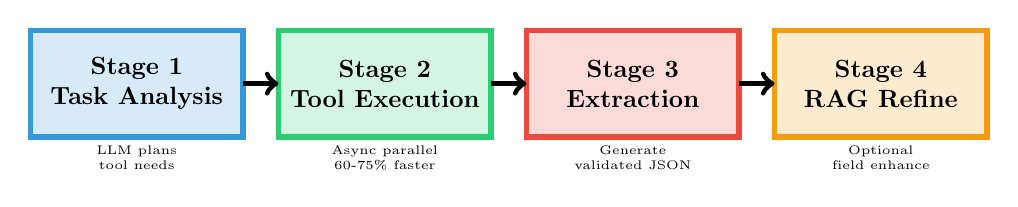
\begin{tikzpicture}[scale=0.9, every node/.style={transform shape}]
    % Boxes
    \draw[fill=clinblue!20, draw=clinblue, line width=2pt] (0,0) rectangle (3,1.5);
    \node[align=center, font=\bfseries] at (1.5,0.75) {Stage 1\\Task Analysis};

    \draw[fill=clingreen!20, draw=clingreen, line width=2pt] (3.5,0) rectangle (6.5,1.5);
    \node[align=center, font=\bfseries] at (5,0.75) {Stage 2\\Tool Execution};

    \draw[fill=clinred!20, draw=clinred, line width=2pt] (7,0) rectangle (10,1.5);
    \node[align=center, font=\bfseries] at (8.5,0.75) {Stage 3\\Extraction};

    \draw[fill=clinorange!20, draw=clinorange, line width=2pt] (10.5,0) rectangle (13.5,1.5);
    \node[align=center, font=\bfseries] at (12,0.75) {Stage 4\\RAG Refine};

    % Arrows
    \draw[->,line width=2pt] (3,0.75) -- (3.5,0.75);
    \draw[->,line width=2pt] (6.5,0.75) -- (7,0.75);
    \draw[->,line width=2pt] (10,0.75) -- (10.5,0.75);

    % Details below
    \node[align=center, font=\tiny] at (1.5,-0.3) {LLM plans\\tool needs};
    \node[align=center, font=\tiny] at (5,-0.3) {Async parallel\\60-75\% faster};
    \node[align=center, font=\tiny] at (8.5,-0.3) {Generate\\validated JSON};
    \node[align=center, font=\tiny] at (12,-0.3) {Optional\\field enhance};
\end{tikzpicture}

\vspace{0.5cm}
\textbf{Key Features:}
\begin{itemize}
    \item Predictable, repeatable execution
    \item Async tool execution (massive speedup)
    \item Automatic adaptive retry on failures
    \item Tool deduplication prevents redundancy
\end{itemize}
\end{frame}

\begin{frame}{ADAPTIVE Mode: Autonomous Loop}
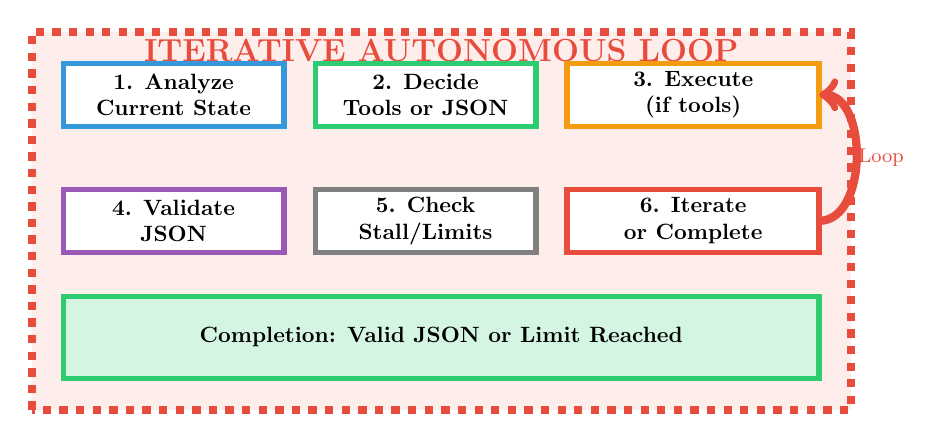
\begin{tikzpicture}[scale=0.8, every node/.style={transform shape}]
    % Main loop box
    \draw[fill=clinred!10, draw=clinred, line width=3pt, dashed] (0,0) rectangle (13,6);
    \node[anchor=north, font=\Large\bfseries, text=clinred] at (6.5,6) {ITERATIVE AUTONOMOUS LOOP};

    % Steps in loop
    \draw[fill=white, draw=clinblue, line width=2pt] (0.5,4.5) rectangle (4,5.5);
    \node[align=center, font=\bfseries] at (2.25,5) {1. Analyze\\Current State};

    \draw[fill=white, draw=clingreen, line width=2pt] (4.5,4.5) rectangle (8,5.5);
    \node[align=center, font=\bfseries] at (6.25,5) {2. Decide\\Tools or JSON};

    \draw[fill=white, draw=clinorange, line width=2pt] (8.5,4.5) rectangle (12.5,5.5);
    \node[align=center, font=\bfseries] at (10.5,5) {3. Execute\\(if tools)};

    \draw[fill=white, draw=clinpurple, line width=2pt] (0.5,2.5) rectangle (4,3.5);
    \node[align=center, font=\bfseries] at (2.25,3) {4. Validate\\JSON};

    \draw[fill=white, draw=gray, line width=2pt] (4.5,2.5) rectangle (8,3.5);
    \node[align=center, font=\bfseries] at (6.25,3) {5. Check\\Stall/Limits};

    \draw[fill=white, draw=clinred, line width=2pt] (8.5,2.5) rectangle (12.5,3.5);
    \node[align=center, font=\bfseries] at (10.5,3) {6. Iterate\\or Complete};

    % Loop arrow
    \draw[->,line width=3pt,clinred] (12.5,3) to[out=0,in=0] (12.5,5);
    \node[anchor=west, font=\small, text=clinred] at (13,4) {Loop};

    % Bottom box
    \draw[fill=clingreen!20, draw=clingreen, line width=2pt] (0.5,0.5) rectangle (12.5,1.8);
    \node[align=center, font=\bfseries] at (6.5,1.15) {Completion: Valid JSON or Limit Reached};
\end{tikzpicture}

\vspace{0.2cm}
\textbf{Max Iterations:} 10 (configurable) | \textbf{Max Tool Calls:} 100 (cost protection)
\end{frame}

% ========================================
% SECTION 4: TOOL SYSTEMS
% ========================================
\section{Tool Systems}

\begin{frame}{Multi-Tool Integration}
\begin{columns}[T]
\column{0.5\textwidth}
\textbf{Functions (40+ Medical Calculations):}
\begin{itemize}
    \item \textcolor{clinblue}{Anthropometry}: BMI, BSA, IBW, growth percentiles, z-scores
    \item \textcolor{clingreen}{Clinical Scores}: HEART, TIMI, CAGE, PHQ-9, SOFA, NIHSS
    \item \textcolor{clinorange}{Lab Calculations}: Corrected Ca, anion gap, CrCl
    \item \textcolor{clinpurple}{Unit Conversions}: kg↔lbs, cm↔inches
    \item \textcolor{gray}{Disease Staging}: AKI (KDIGO), COPD (GOLD)
\end{itemize}

\column{0.5\textwidth}
\textbf{Patterns (33+ Text Normalizations):}
\begin{itemize}
    \item Vital signs: BP, HR, RR, SpO2, Temp
    \item Lab values: Glucose, HbA1c, electrolytes
    \item Medications: Dosing, frequency, routes
    \item Abbreviations: DM→Diabetes Mellitus
\end{itemize}

\vspace{0.3cm}
\textbf{Extras (49+ Clinical Hints):}
\begin{itemize}
    \item Growth standards (WHO, CDC)
    \item Malnutrition criteria (ASPEN)
    \item Diagnostic criteria
    \item Assessment scales
\end{itemize}
\end{columns}
\end{frame}

\begin{frame}{Tool Execution: Autonomous Orchestration}
\textbf{LLM Autonomously Decides:}
\begin{enumerate}
    \item \textcolor{clinblue}{Which tools are needed?} (based on task description)
    \item \textcolor{clingreen}{What parameters to extract?} (from clinical text)
    \item \textcolor{clinorange}{How to compose results?} (function chaining supported)
\end{enumerate}

\vspace{0.3cm}
\begin{exampleblock}{Example: Pediatric Malnutrition Assessment}
\small
\textbf{Input:} "6-year-old, weight 16kg, height 110cm"\\[0.2cm]
\textbf{LLM Autonomously Calls:}
\begin{itemize}
    \item \texttt{calculate\_bmi(16, 1.1)} → 13.2
    \item \texttt{calculate\_growth\_percentile(72, 13.2, 'bmi')} → -2.1 SD
    \item \texttt{interpret\_zscore\_malnutrition(-2.1)} → "Moderate wasting"
    \item RAG: Retrieve ASPEN malnutrition criteria
\end{itemize}
\textbf{Output:} Structured diagnosis with evidence
\end{exampleblock}
\end{frame}

% ========================================
% SECTION 5: PERFORMANCE OPTIMIZATIONS
% ========================================
\section{Performance Optimizations}

\begin{frame}{Production-Ready Performance}
\begin{table}
\small
\begin{tabular}{p{4cm}|p{3.5cm}|p{4.5cm}}
\toprule
\textbf{Optimization} & \textbf{Speedup} & \textbf{Implementation} \\
\midrule
LLM Response Cache & \textcolor{clingreen}{\textbf{400x faster}} & SQLite DB, hash-based keys \\
Async Tool Execution & \textcolor{clingreen}{\textbf{60-75\% faster}} & asyncio.gather() parallel \\
Batch Preprocessing & \textcolor{clingreen}{\textbf{15-25\% faster}} & Single-pass PHI + patterns \\
Multi-GPU Processing & \textcolor{clingreen}{\textbf{2-4x faster}} & ProcessPoolExecutor (local) \\
Parallel Batch Process & \textcolor{clingreen}{\textbf{5-10x faster}} & ThreadPoolExecutor (cloud) \\
\bottomrule
\end{tabular}
\end{table}

\vspace{0.3cm}
\textbf{Adaptive Retry System:}
\begin{itemize}
    \item Progressive context reduction: 100\% → 80\% → 60\% → 40\% → 20\%
    \item Automatic minimal prompt fallback
    \item Exponential backoff for transient errors
    \item Provider-specific strategies (OpenAI, Claude, Gemini, local)
\end{itemize}
\end{frame}

\begin{frame}[fragile]{Cache Mechanism}
\textbf{Hash-Based LLM Response Caching:}
\begin{lstlisting}[language=Python]
def _compute_cache_key(self, prompt):
    hash_input = (
        prompt +
        self.model_name +
        str(self.temperature) +
        self.prompt_config_hash  # Auto-invalidates
    )
    return hashlib.md5(hash_input.encode()).hexdigest()

if cache_key in cache:
    return cache[cache_key]  # 0.5ms vs 200ms API call
\end{lstlisting}

\vspace{0.3cm}
\textbf{Benefits:}
\begin{itemize}
    \item Identical prompts return instantly (testing, re-runs)
    \item Automatic invalidation when config changes
    \item Saves \$\$\$ on API costs
\end{itemize}
\end{frame}

% ========================================
% SECTION 6: USE CASES
% ========================================
\section{Capabilities \& Use Cases}

\begin{frame}{Universal Platform - Not Limited to Examples}
\begin{block}{Platform is Task-Agnostic}
\textbf{Any clinical task} you define through prompts, schemas, and tools
\end{block}

\begin{columns}[T]
\column{0.5\textwidth}
\textbf{Demonstrated Use Cases:}
\begin{itemize}
    \item Clinical classification (ADRD, malnutrition)
    \item Data extraction \& curation
    \item Chart review automation
    \item Quality improvement metrics
    \item Research data collection
    \item Clinical decision support
    \item Comprehensive annotation
\end{itemize}

\column{0.5\textwidth}
\textbf{Potential Applications:}
\begin{itemize}
    \item Risk stratification
    \item Medication reconciliation
    \item Clinical trial screening
    \item Adverse event detection
    \item Guideline compliance
    \item Disease surveillance
    \item Registry reporting
\end{itemize}
\end{columns}

\vspace{0.4cm}
\centering
\fbox{\parbox{0.85\textwidth}{\centering
\textbf{The only limit is your task description} - not the platform
}}
\end{frame}

\begin{frame}{Multi-Column Prompt Variables (v1.0.0)}
\textbf{Pass ANY dataset columns as template variables:}

\begin{exampleblock}{Example}
\small
\textbf{CSV Columns:} patient\_id, age, gender, admission\_type, clinical\_text\\[0.2cm]
\textbf{Prompt Template:}\\
\texttt{"Extract diagnosis for patient \{patient\_id\}, \{age\}yo \{gender\},\\
admitted for \{admission\_type\}: \{clinical\_text\}"}\\[0.2cm]
\textbf{Rendered for Row 1:}\\
\texttt{"Extract diagnosis for patient 12345, 65yo M,\\
admitted for Emergency: [clinical text here]"}
\end{exampleblock}

\vspace{0.3cm}
\textbf{Benefits:}
\begin{itemize}
    \item Richer context for LLM (age-appropriate norms, gender-specific ranges)
    \item No hardcoding - fully configurable via UI
    \item Backward compatible (text-only mode still supported)
\end{itemize}
\end{frame}

% ========================================
% SECTION 7: TECHNICAL HIGHLIGHTS
% ========================================
\section{Technical Highlights}

\begin{frame}{Multi-Provider LLM Support}
\begin{table}
\small
\begin{tabular}{p{3cm}|p{5cm}|p{4cm}}
\toprule
\textbf{Provider} & \textbf{Models} & \textbf{Notes} \\
\midrule
OpenAI & GPT-4, GPT-4o, o1-preview/mini & Native function calling \\
Anthropic & Claude 3.5 Sonnet, Opus, Haiku & 200K context window \\
Google & Gemini 1.5 Pro, Flash & Long-context specialist \\
Azure OpenAI & Enterprise deployments & HIPAA-compliant \\
Local (Unsloth) & Llama, Phi, Qwen, Mistral & Multi-GPU support \\
\bottomrule
\end{tabular}
\end{table}

\vspace{0.3cm}
\textbf{Unified Interface:}
\begin{itemize}
    \item Adapter pattern - swap providers without code changes
    \item Model-specific optimizations (chat templates, token limits)
    \item Provider-specific adaptive retry strategies
\end{itemize}
\end{frame}

\begin{frame}{RAG Engine Architecture}
\textbf{Retrieval-Augmented Generation for Clinical Guidelines:}

\begin{columns}[T]
\column{0.5\textwidth}
\textbf{Document Ingestion:}
\begin{itemize}
    \item PDF, URL, text file support
    \item Automatic chunking (512 chars, 50 overlap)
    \item Batch embedding (25-40\% faster)
    \item FAISS vector storage (CPU/GPU)
\end{itemize}

\vspace{0.2cm}
\textbf{Retrieval:}
\begin{itemize}
    \item Cosine similarity search
    \item Top-K retrieval (configurable)
    \item Source citation tracking
    \item Cache for embeddings
\end{itemize}

\column{0.5\textwidth}
\textbf{Two Integration Points:}
\begin{enumerate}
    \item \textcolor{clinblue}{Stage 2 (STRUCTURED)} or \textcolor{clinblue}{Step 3A (ADAPTIVE)}:\\
    General knowledge retrieval based on clinical text

    \vspace{0.3cm}
    \item \textcolor{clinorange}{Stage 4 (STRUCTURED only)}:\\
    Field-specific refinement with evidence and citations
\end{enumerate}

\vspace{0.2cm}
\textbf{Embedding Model:}\\
\texttt{sentence-transformers/all-mpnet-base-v2}
\end{columns}
\end{frame}

\begin{frame}{Security \& Compliance}
\textbf{PHI Redaction Engine:}
\begin{itemize}
    \item Detect \& redact: Dates, Names, IDs, Locations, Phone, Email, SSN, MRN
    \item Configurable redaction methods:
    \begin{itemize}
        \item Replace with tag: "[DATE]", "[NAME]", "[ID]"
        \item Remove completely
        \item Mask with asterisks
    \end{itemize}
    \item Optional: Save redacted text column in output
\end{itemize}

\vspace{0.3cm}
\textbf{Data Processing:}
\begin{itemize}
    \item Local execution - data never leaves your environment
    \item Support for on-premise LLMs (Unsloth/local models)
    \item Azure OpenAI for HIPAA-compliant cloud deployments
    \item Detailed audit logging
\end{itemize}
\end{frame}

% ========================================
% SECTION 8: RESULTS & VALIDATION
% ========================================
\section{Results \& Validation}

\begin{frame}{Performance Benchmarks}
\textbf{Malnutrition Classification (200 EHR notes):}
\begin{table}
\small
\begin{tabular}{l|c|c|c}
\toprule
\textbf{Metric} & \textbf{No Optimization} & \textbf{With Optimization} & \textbf{Speedup} \\
\midrule
Total Time & 45 minutes & 6 minutes & \textcolor{clingreen}{\textbf{7.5x}} \\
Per-row Time & 13.5s & 1.8s & \textcolor{clingreen}{\textbf{7.5x}} \\
Cache Hits & 0\% & 65\% & \textcolor{clingreen}{\textbf{400x on hits}} \\
API Calls & 600 & 210 & 65\% reduction \\
Cost (GPT-4) & \$18.50 & \$6.45 & 65\% savings \\
\bottomrule
\end{tabular}
\end{table}

\vspace{0.3cm}
\textbf{Configuration:}
\begin{itemize}
    \item LLM Cache: Enabled
    \item Async Tool Execution: Enabled
    \item Batch Preprocessing: Enabled
    \item Parallel Processing: 4 workers (cloud API)
\end{itemize}
\end{frame}

\begin{frame}{Multi-GPU Performance (Local Models)}
\textbf{MIMIC-IV Diagnosis Annotation (1000 discharge summaries):}
\begin{table}
\small
\begin{tabular}{l|c|c|c}
\toprule
\textbf{Configuration} & \textbf{Time} & \textbf{Throughput} & \textbf{Speedup} \\
\midrule
Single GPU (H100) & 120 min & 8.3 docs/min & 1.0x \\
2 GPUs (H100) & 65 min & 15.4 docs/min & \textcolor{clingreen}{\textbf{1.85x}} \\
4 GPUs (H100) & 38 min & 26.3 docs/min & \textcolor{clingreen}{\textbf{3.16x}} \\
8 GPUs (H100) & 25 min & 40.0 docs/min & \textcolor{clingreen}{\textbf{4.8x}} \\
\bottomrule
\end{tabular}
\end{table}

\vspace{0.3cm}
\textbf{Model:} Llama-3.1-8B-Instruct (4-bit quantized)\\
\textbf{Processing:} ProcessPoolExecutor (process-based parallelism, safe for CUDA)
\end{frame}

% ========================================
% SECTION 9: DEPLOYMENT
% ========================================
\section{Deployment \& Usage}

\begin{frame}[fragile]{Installation \& Setup}
\textbf{From PyPI:}
\begin{lstlisting}[language=bash]
pip install clinorchestra

# With local LLM support
pip install clinorchestra[local]
\end{lstlisting}

\vspace{0.3cm}
\textbf{Launch Application:}
\begin{lstlisting}[language=bash]
clinorchestra
# Opens at http://localhost:7860
\end{lstlisting}

\vspace{0.3cm}
\textbf{Programmatic Usage (Python SDK):}
\begin{lstlisting}[language=Python]
from clinorchestra import AppState, create_agent

# Configure
app_state = AppState()
app_state.set_model_config(...)
app_state.set_prompt_config(...)

# Process
agent = create_agent(app_state)
result = agent.extract(clinical_text)
\end{lstlisting}
\end{frame}

\begin{frame}{Basic Workflow}
\begin{enumerate}
    \item \textbf{Model Setup}: Select LLM provider, configure API keys
    \item \textbf{Define Task}: Write extraction prompt and JSON schema
    \item \textbf{Upload Data}: Load CSV file with clinical text
    \item \textbf{Configure Tools}:
    \begin{itemize}
        \item Enable patterns for text normalization
        \item Enable functions for medical calculations
        \item Add extras for domain knowledge
        \item Upload RAG documents for guidelines
    \end{itemize}
    \item \textbf{Test}: Use Playground to test single extraction
    \item \textbf{Process}: Batch process entire dataset
    \item \textbf{Export}: Download results CSV with structured extractions
\end{enumerate}

\vspace{0.3cm}
\begin{alertblock}{Documentation}
Complete guides: \texttt{SDK\_GUIDE.md}, \texttt{ARCHITECTURE.md}, \texttt{MULTI\_GPU\_GUIDE.md}
\end{alertblock}
\end{frame}

% ========================================
% SECTION 10: CONCLUSIONS
% ========================================
\section{Conclusions \& Future Work}

\begin{frame}{Key Contributions}
\begin{enumerate}
    \item \textbf{Universal Platform Architecture}
    \begin{itemize}
        \item Task-driven, not task-specific
        \item Adapts to ANY clinical task through LLM orchestration
        \item No hardcoded logic - fully user-configurable
    \end{itemize}

    \vspace{0.2cm}
    \item \textbf{Dual Execution Modes}
    \begin{itemize}
        \item STRUCTURED: 4-stage pipeline for production scale
        \item ADAPTIVE: Iterative autonomous loop for complex cases
        \item Runtime selection based on task requirements
    \end{itemize}

    \vspace{0.2cm}
    \item \textbf{Production-Ready Performance}
    \begin{itemize}
        \item 400x cache speedup, 60-75\% async gains
        \item Multi-GPU support (2-4x on H100 clusters)
        \item Robust error handling (adaptive retry, fallback)
    \end{itemize}

    \vspace{0.2cm}
    \item \textbf{Comprehensive Tool Integration}
    \begin{itemize}
        \item 40+ functions, 33+ patterns, 49+ extras, RAG
        \item Autonomous tool orchestration by LLM
        \item Plugin architecture for extensibility
    \end{itemize}
\end{enumerate}
\end{frame}

\begin{frame}{Future Directions}
\begin{columns}[T]
\column{0.5\textwidth}
\textbf{Technical Enhancements:}
\begin{itemize}
    \item Streaming responses for real-time feedback
    \item Graph-based RAG for structured knowledge
    \item Multi-agent collaboration
    \item Vision model support (PDF images)
    \item Active learning for schema refinement
\end{itemize}

\column{0.5\textwidth}
\textbf{Domain Extensions:}
\begin{itemize}
    \item ICD-10/CPT coding
    \item Drug-drug interaction checking
    \item Temporal reasoning (disease progression)
    \item Multi-document synthesis
    \item Comparative effectiveness analysis
\end{itemize}
\end{columns}

\vspace{0.4cm}
\textbf{Validation \& Evaluation:}
\begin{itemize}
    \item Large-scale benchmarking on public datasets
    \item Inter-rater reliability studies
    \item Clinical workflow integration pilots
    \item Cost-effectiveness analysis
\end{itemize}
\end{frame}

\begin{frame}{Impact \& Applications}
\begin{block}{Transforming Clinical Data Science}
\textbf{From manual curation to autonomous AI orchestration}
\end{block}

\vspace{0.3cm}
\textbf{Potential Impact:}
\begin{itemize}
    \item \textcolor{clingreen}{Accelerate clinical research} (months → days for dataset curation)
    \item \textcolor{clinblue}{Improve data quality} (consistent, evidence-based extractions)
    \item \textcolor{clinorange}{Reduce costs} (automation + caching saves \$\$\$)
    \item \textcolor{clinpurple}{Enable new analyses} (large-scale EHR mining now feasible)
    \item \textcolor{clinred}{Democratize access} (open-source, user-friendly)
\end{itemize}

\vspace{0.3cm}
\begin{exampleblock}{Vision}
\textbf{Universal clinical AI infrastructure} - not a single-purpose tool, but a platform that adapts to \textit{any} clinical data extraction task through autonomous LLM orchestration
\end{exampleblock}
\end{frame}

% Final Frame
\begin{frame}[standout]
\Huge\textbf{Thank You!}

\vspace{1cm}
\Large
\textbf{ClinOrchestra v1.0.0}\\
\large
Universal, Autonomous Clinical AI Platform

\vspace{0.5cm}
\normalsize
Frederick Gyasi\\
\texttt{gyasi@musc.edu}\\[0.2cm]
Medical University of South Carolina\\
Biomedical Informatics Center

\vspace{0.5cm}
\small
\textbf{GitHub:} \texttt{https://github.com/gyasifred/clinorchestra}\\
\textbf{Documentation:} \texttt{SDK\_GUIDE.md}, \texttt{ARCHITECTURE.md}
\end{frame}

\end{document}
